%%%%%%%%%%%%%%%%%%%%%%%%%%%%%%%%%%%%%%%%%%%%%%%%%%%%%%%%%%%%%%%%%%%%%%%%%%%%%%%%
%2345678901234567890123456789012345678901234567890123456789012345678901234567890
%        1         2         3         4         5         6         7         8

\documentclass[letterpaper, 10 pt, conference]{ieeeconf}  % Comment this line out if you need a4paper

\usepackage{graphicx}% so it makes black blobs
\graphicspath{ {imgs/} }
% \usepackage{hyperref}
\usepackage{amsmath}
% \usepackage{usenix,epsfig,endnotes}
% \usepackage{graphicx}


%\documentclass[a4paper, 10pt, conference]{ieeeconf}      % Use this line for a4 paper

\IEEEoverridecommandlockouts                              % This command is only needed if 
                                                          % you want to use the \thanks command

\overrideIEEEmargins                                      % Needed to meet printer requirements.

% See the \addtolength command later in the file to balance the column lengths
% on the last page of the document

% The following packages can be found on http:\\www.ctan.org
%\usepackage{graphics} % for pdf, bitmapped graphics files
%\usepackage{epsfig} % for postscript graphics files
%\usepackage{mathptmx} % assumes new font selection scheme installed
%\usepackage{times} % assumes new font selection scheme installed
%\usepackage{amsmath} % assumes amsmath package installed
%\usepackage{amssymb}  % assumes amsmath package installed

\title{\LARGE \bf
3D Dense Mapping and Localization with ICP
}


\author{
{\rm Yiren Lu}\\
GRASP Lab, University of Pennsylvania\\
May 2016
}
% \author{Albert Author$^{1}$ and Bernard D. Researcher$^{2}$% <-this % stops a space
% \thanks{*This work was not supported by any organization}% <-this % stops a space
% \thanks{$^{1}$Albert Author is with Faculty of Electrical Engineering, Mathematics and Computer Science,
%         University of Twente, 7500 AE Enschede, The Netherlands
%         {\tt\small albert.author@papercept.net}}%
% \thanks{$^{2}$Bernard D. Researcheris with the Department of Electrical Engineering, Wright State University,
%         Dayton, OH 45435, USA
%         {\tt\small b.d.researcher@ieee.org}}%
% }


\begin{document}



\maketitle
\thispagestyle{empty}
\pagestyle{empty}


%%%%%%%%%%%%%%%%%%%%%%%%%%%%%%%%%%%%%%%%%%%%%%%%%%%%%%%%%%%%%%%%%%%%%%%%%%%%%%%%
\begin{abstract}

Iterative Closest Point (ICP) is widely used in 3D models registration and robotics localization and mapping. In this project, I investaged variations of ICP pipeline and implemented a highly efficient and optimized ICP in order to do localization and mapping task. We were provided with RGB-D data of an Xtion installed on a moving quadrone as well as the Vicon's data as ground truth. In this report, I will describe my approach and present the final results.\\

\end{abstract}


%%%%%%%%%%%%%%%%%%%%%%%%%%%%%%%%%%%%%%%%%%%%%%%%%%%%%%%%%%%%%%%%%%%%%%%%%%%%%%%%
\section{INTRODUCTION}

Iterative Closest Point (ICP) is an algorithm employed to minimize the difference between two clouds of points. ICP is often used to reconstruct 2D or 3D surfaces from different scans, to localize robots and achieve optimal path planning (especially when wheel odometry is unreliable). In this project, I did 3D dense mapping and location with only RGB-D data. I investigated the standard pipe of the ICP algorithm as well as various variations \cite{c1} \cite{c2} of ICP that could significantly improve the performance or efficiency. I then implemented a highly optimized version of ICP which could reconstruct the 3D scene and localize the robot in real-time. In the following report, I will decribe in details of my approach and the pros and cons of various approaches I have tried.\\

\section{RGB-D Data Preprocessing}
\subsection{Mapping to 3D Euclidean Space}
I first mapped the RGBD images back to 3D Euclidean spaces using depth images. \\
$$
Y = D/1000
$$
$$
X = (U - \mbox{offsetX})/f_{x}
$$
$$
Z = -(V-\mbox{offsetY})/f_{y}
$$
Where, $(U,V,D)$ are the depth image points. $(X,Y,Z)$ are the mapped points in Euclidean space. offsetX, offsetY, $f_x, f_y$ are given from the calibration matrix.\\
\subsection{Computing the Normals}
Since later in ICP, there are multiple steps involving normals of each sampled points, I first compute the normals. For each point, first, select 4-nearest neighbour from the model. (Here, more points will give more robust normals estimation, which also requires more computation.) And then do Princple Component Analysis (PCA) of the selected 5 points using Singular Value Decomposition (SVD). And finally select the eigen vector corresponding to the smallest eigenvalues as the normal.\\
Note that here, I employed K-d tree to accelerate the computing of k-nearest neighbor. In the later computation of KNN, I also adopted K-d tree.\\
\section{Iterative Closest Point}
The standard pipeline of ICP is A) Sampling B) Matching C) Weighting & Rejection E) Optimization. 
\subsection{Sampling}
The most common way of sampling is 1) Using all available points 2) Uniform Sampling 3) Random Sampling. 1) takes too much computation. Also sparse representation that captures features actually outperforms using all available points. 2) and 3) have similar performance. I then adopted normals-space sampling technique described in \cite{c1}, which improve the performance by a considerable amount. \\
The idea of normals-space sampling is to sample more points where the normals changes much. It is a simple approach to exploit model features. Figure \ref{fig:nspace}. First, I convert the 3D normals into spherical coordinates, which are represented in 2d. I then binning uniformly of all the normals. (We can also do kmeans, which involves more computation.) And finally sample uniformly from bins with at least one normal.\\
\begin{figure}
\centering
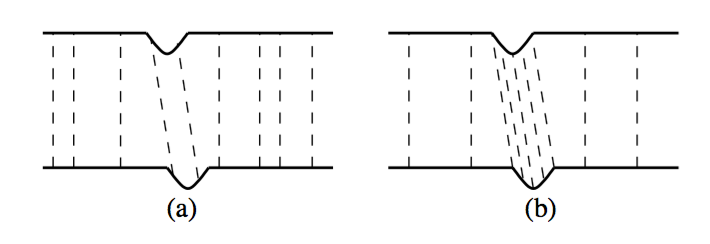
\includegraphics[width=\columnwidth]{normalspace.png}\\
\caption{(a) Random sampling (b) Normal-space sampling}
\label{fig:nspace}
\end{figure}
\subsection{Matching}

Matching is an important step of ICP. If we can find the optimal matching between the two models, we can solve the registration problem analytically. Here for matching I incorporated RGB values into the nearest neighbor criterion. I did KNN search leveraging K-D tree.\\

\subsection{Weighting \& Rejection}
I assigned uniform weights to the matched pairs and adopted two rejection method. 1) Normal incompatibility, 2) Rejecting boundary points. For 1) I rejected the matched pairs with their normals angle greater 45 degree. For 2), since the quadrone viewport is moving, the two models are always partially overlapped, trimming the boundaries significantly improves the alignment performance and also reduces the computation.\\
\subsection{Optimization Metric}
For the optimization metric, I did both 1) standard least squars approximation and the 2) point to plane error optimization. \\
1) is described in \cite{c3}. Suppose $S_{3\times n}$ is the set of the source points, $D_{3\times n}$ is the set of the target points, we want to find rotation matrix $R_{3\times 3}$ and tranlation vector $T_{3\times 1}$, such that \\
\begin{align*}
\sum_{i=1}^N ||D_i - (RS_i + T)||_2\\
\end{align*}
is minimized. Where $D_i$ is the $i$th column in $D$, $S_i$ is the $i$th column in $S$. Following the paper, first compute $H = SD^T$. And then find the SVD of $H$: $H = U\Lambda V^T$. And finally, $R = VU^T$, $T = \sum_i(D_i-RS_i)/n$.\\
2) is described in \cite{c2} and illustrated in figure \ref{fig:p2p}.
\begin{figure}
\centering
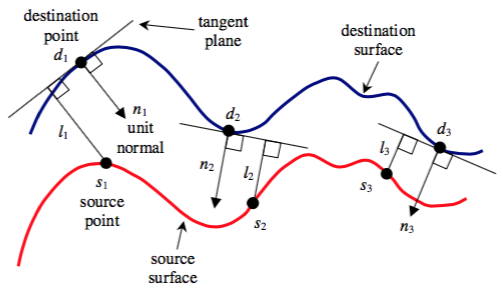
\includegraphics[width=\columnwidth]{p2plane.png}\\
\caption{Point to plane error}
\label{fig:p2p}
\end{figure}
Suppose $N_{3\times n}$ are the normals of the destination points. To evaluate $R$ and $T$ with point-to-plane error metric. The procedure is as follows\\
\begin{align*}
b =& (D-S)\bullet N\\
A =& [S\times n, N]\\
x =& A^{\dagger} b\\
\end{align*}
Where, $\bullet$ is the dot product. $\times$ is the cross product. $A^\dagger$ is the pysuedo-inverse of $A$. (Note, psyuedo-inverse could be efficiently done by SVD). $x = (\alpha, \beta, \gamma, t_x, t_y, t_z)$.\\
\begin{align*}
R =& R_z(\gamma)R_y(\beta)R_x(\alpha)\\
T =& [t_x, t_y, t_z]^T\\
\end{align*}
By experiment, point-to-plane metric works slightly better than standard least squares.\\
\subsection{Summary}
After the above optimization, the ICP works pretty well for my test frame 1 vs frame 50 in dataset 5 and it perfectly generalized into other frame pairs. Some sample videoclips are attached. \\
% b = dot(d-s, n, 2);
% A1 = cross(s, n);
% A2 = Normals;
% A=[A1 A2];
% X = (A\b)';


\section{Mapping and Localization}
For Mapping and Localization, I iteratively applied ICP to the current frame and the previous and compute a relative rotation matrix $R$ and translation vector $T$. And then accumulate the rotation and translation motion by the equation \\
\begin{align*}
R_{t} =& RR_{t-1}\\
T_{t} =& RT_{t-1}+ T_{t-1}\\
\end{align*}
Where, $R_t$ and $T_t$ are the global rotation matrix and translation vector at step $t$. Finally, I map the orientation and location into $(row_t, pitch_t, yaw_t, x_t, y_t, z_t)$, six dimensional vectors for each step $t$. \\
\section{Results and Discussion}

The orientation and location estimation are plotted in figure \ref{fig:loc}. We can see that in general, the orientation estimation is close to the Vicon's data. For the location estimation, the general tendency is right. While, the estimation from ICP has some drifting.\\
I then did 3D reconstruction using both Vicon's and ICP's estimation. The frame-per-second(fps) for only computing ICP is 108.71. Most of the execution time in the demo is on displaying the point cloud. \\
We can see the plotting in figure \ref{fig:viconicp} that, even though we treat Vicon as ground truth, there is some noise for Vicon. In addition, the calibration for the camera seems to be distorted. (See the wrapped ground of figure \ref{fig:viconicp_side}.). Comparing Vicon's reconstruction with ICP's reconstruction, we can see that ICP produced finer model then Vicon's. However, when we look from the top view, due to the distortion of calibration and the cumulated error of ICP, the wall in the ICP's reconstruction is wrapped. \\
To solve this problem, here are some methods that I would do if I got more time
\begin{figure}
\centering
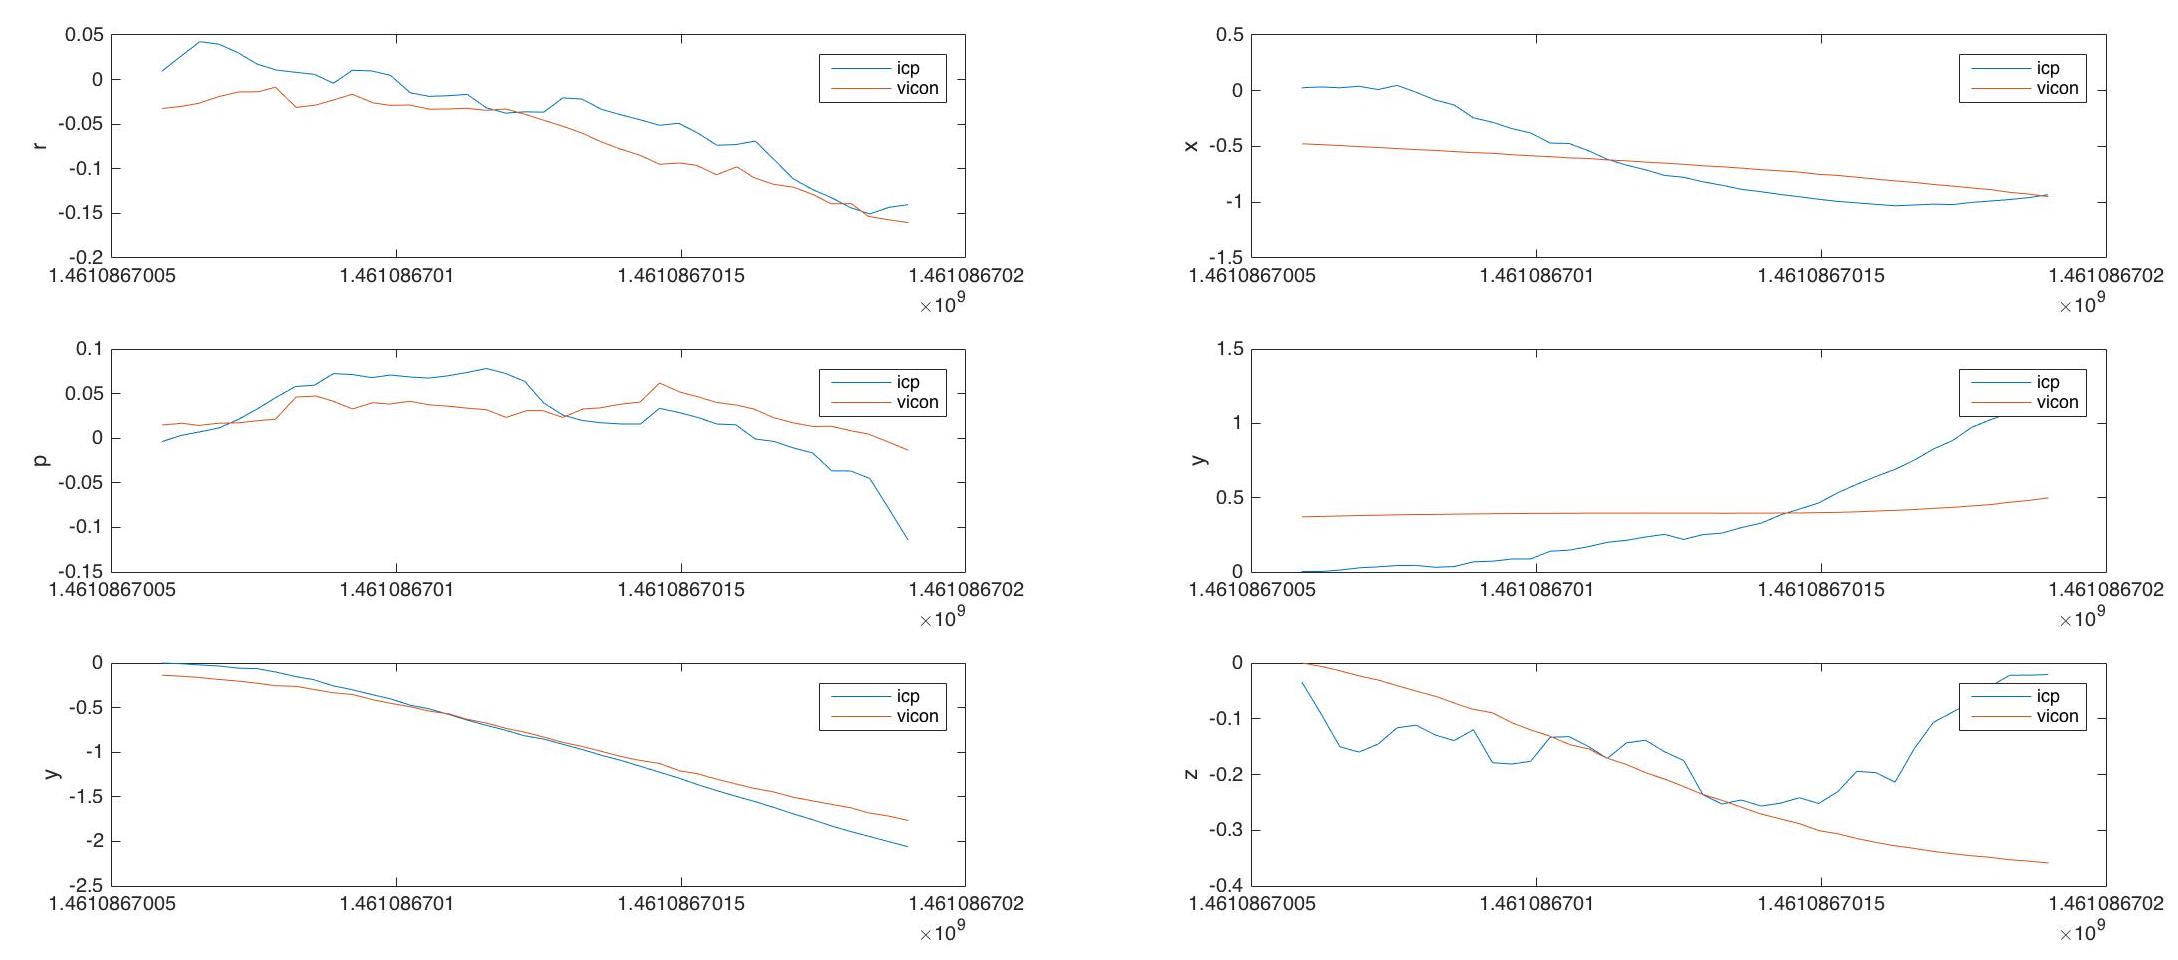
\includegraphics[height=\columnwidth, angle =90 ]{may2localization.jpg}\\
\caption{Orientation and location estimation vs Vicon's data.}
\label{fig:loc}
\end{figure}
\begin{figure}
\centering
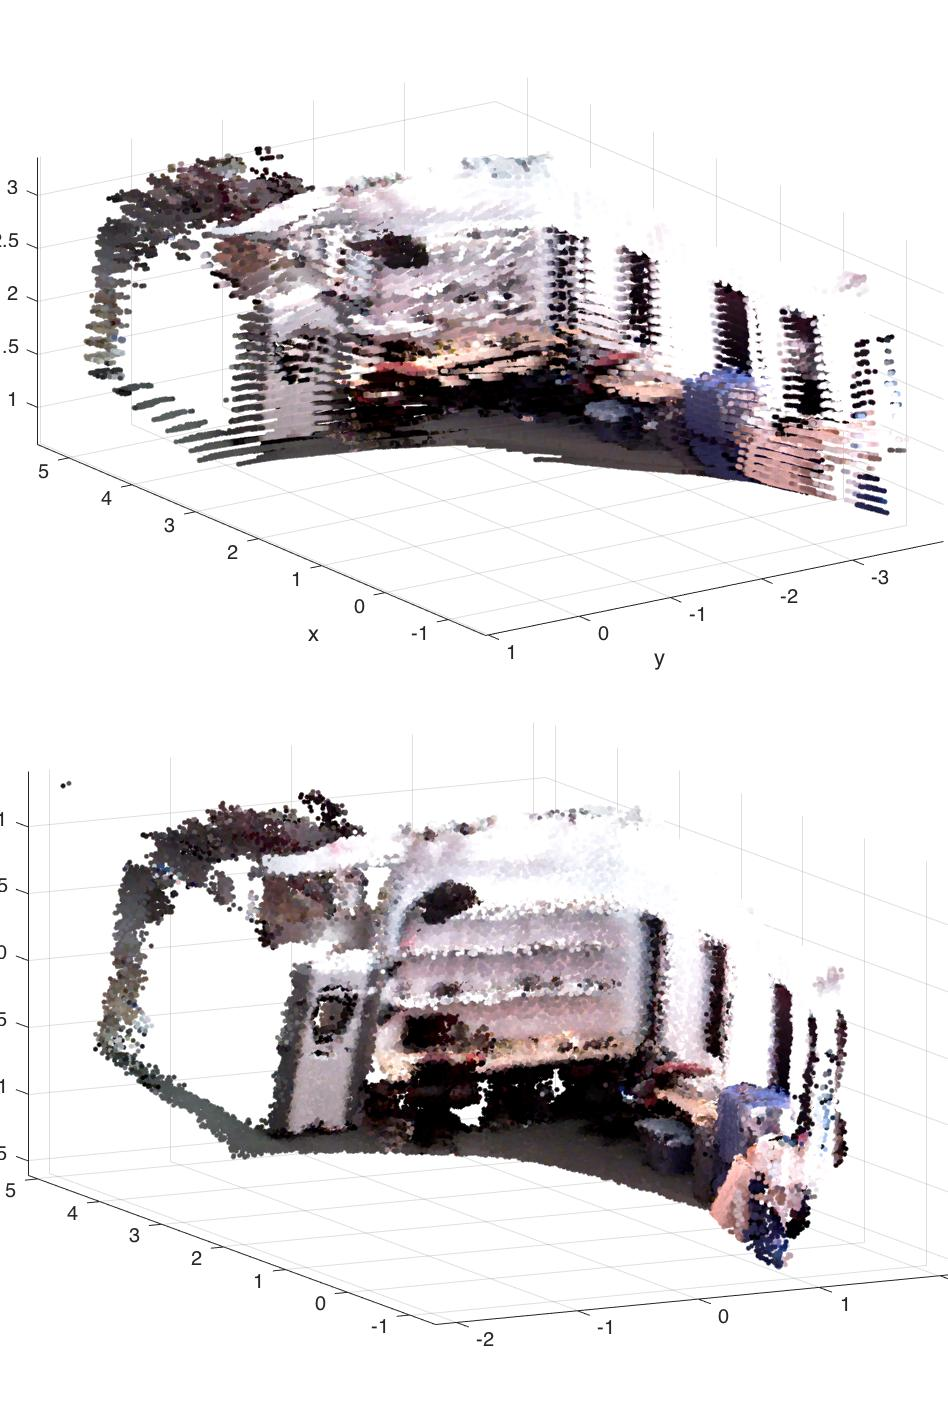
\includegraphics[width=\columnwidth]{viconicp.jpg}\\
\caption{Top: 3D reconstruction from Vicon. Bottom: 3D reconstruction from ICP}
\label{fig:viconicp}
\end{figure}



\begin{itemize}
\item Global registration. i.e., for each frame, using ICP to estimate the $R$ and $T$ against all the previous frames rather than a single previous frame. The error may propagate in my current approach.
\item Obtain better camera calibration. (Maybe using checker board.)
\item Fusing Vicon's data with EKF. 
\item Plane estimation and rejecting outliers. 
\end{itemize}



\addtolength{\textheight}{-12cm}   % This command serves to balance the column lengths
                                  % on the last page of the document manually. It shortens
                                  % the textheight of the last page by a suitable amount.
                                  % This command does not take effect until the next page
                                  % so it should come on the page before the last. Make
                                  % sure that you do not shorten the textheight too much.

%%%%%%%%%%%%%%%%%%%%%%%%%%%%%%%%%%%%%%%%%%%%%%%%%%%%%%%%%%%%%%%%%%%%%%%%%%%%%%%%



%%%%%%%%%%%%%%%%%%%%%%%%%%%%%%%%%%%%%%%%%%%%%%%%%%%%%%%%%%%%%%%%%%%%%%%%%%%%%%%%



\section*{ACKNOWLEDGMENT}

Thanks Dr. Lee for designing and preparing this project and thanks TAs for timely responses to our questions.





\begin{thebibliography}{99}

\bibitem{c1} Rusinkiewicz, Szymon, and Marc Levoy. "Efficient variants of the ICP algorithm." 3-D Digital Imaging and Modeling, 2001. Proceedings. Third International Conference on. IEEE, 2001.
\bibitem{c2} Low, Kok-Lim. "Linear least-squares optimization for point-to-plane icp surface registration." Chapel Hill, University of North Carolina 4 (2004).
\bibitem{c3} Arun, K. Somani, Thomas S. Huang, and Steven D. Blostein. "Least-squares fitting of two 3-D point sets." Pattern Analysis and Machine Intelligence, IEEE Transactions on 5 (1987): 698-700.





\end{thebibliography}



\begin{figure}
\centering
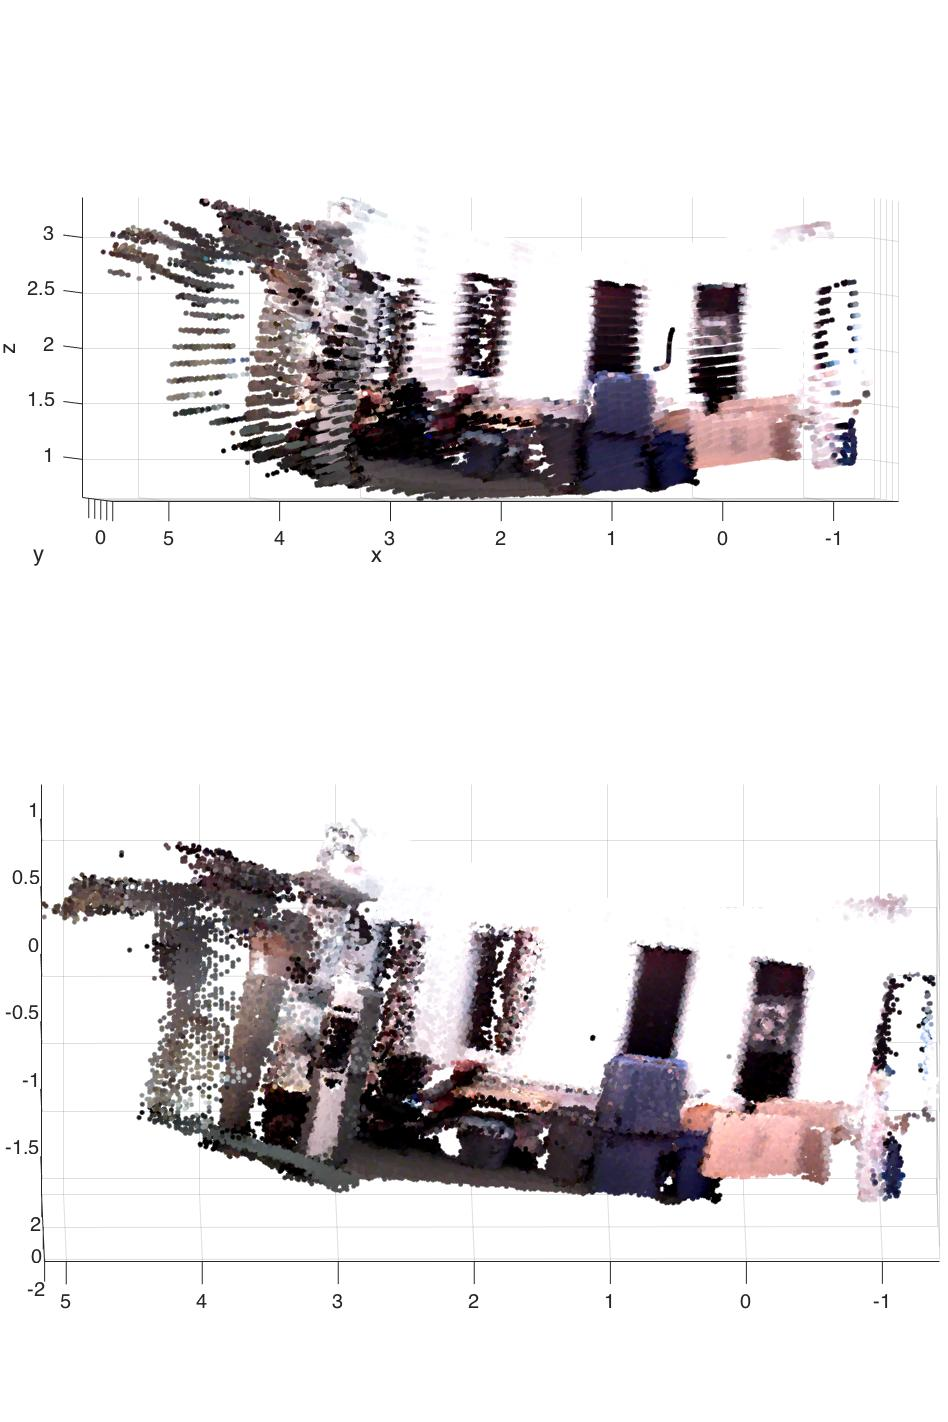
\includegraphics[width=\columnwidth]{viconicp_side.jpg}\\
\caption{Side view. Top: 3D reconstruction from Vicon. Bottom: 3D reconstruction from ICP}
\label{fig:viconicp_side}
\end{figure}

\begin{figure}
\centering
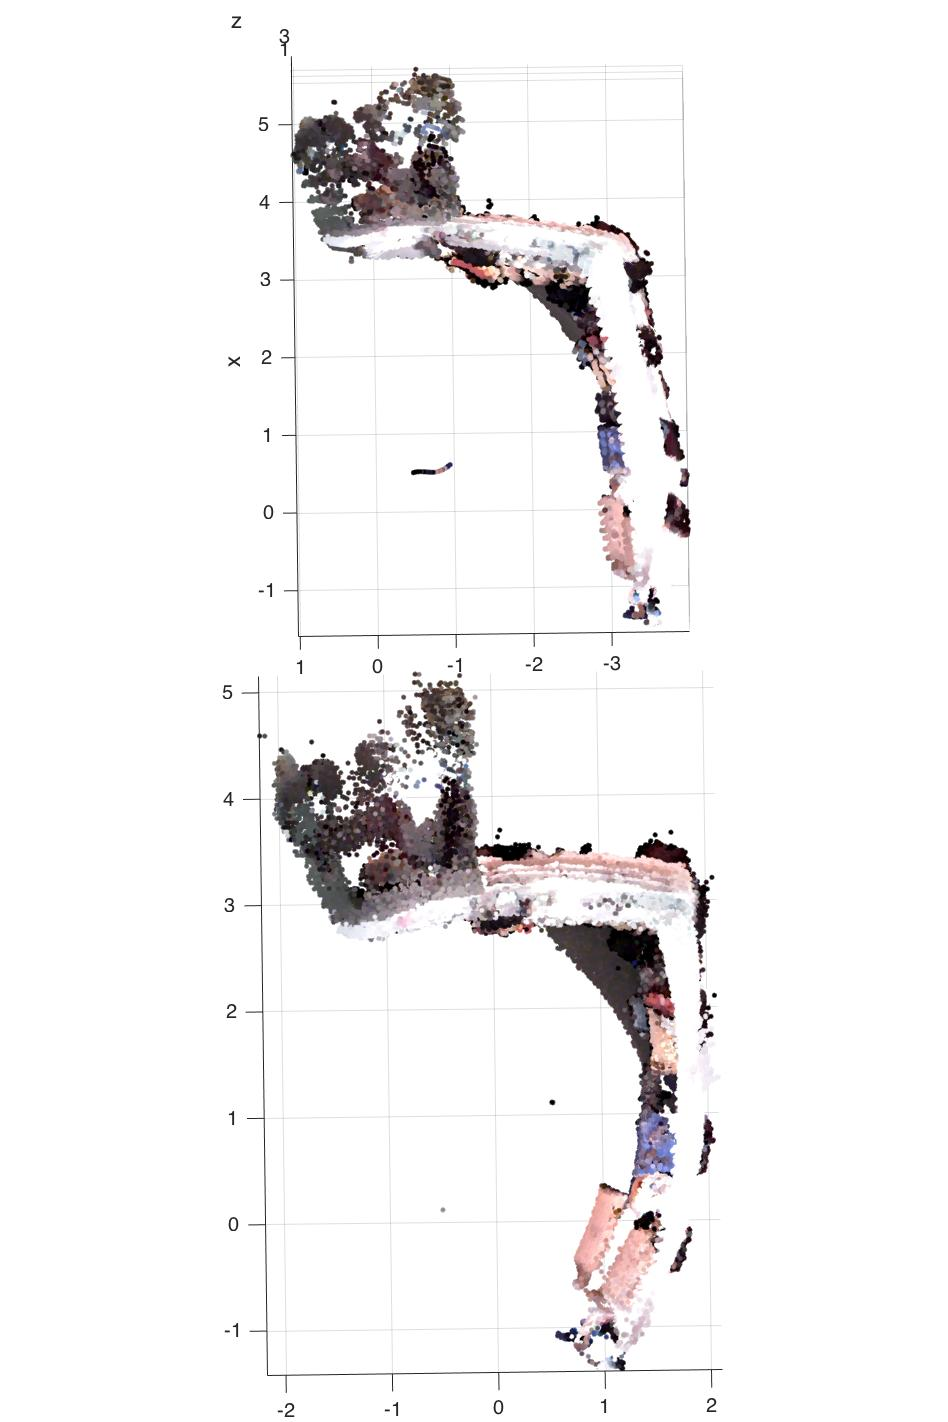
\includegraphics[width=\columnwidth]{viconicp_top.jpg}\\
\caption{Top view. Top: 3D reconstruction from Vicon. Bottom: 3D reconstruction from ICP}
\label{fig:viconicp_side}
\end{figure}

\end{document}
